\chapter{Scope}
\label{ch:scope}

This chapter constitutes a preparatory step before describing the model in the next chapter. On the one hand, this chapter lays out the scope of the project and justifies the main design decisions taken for developing a system. In the other hand, it presents the architectural framework adopted in our system and provides some theoretical background.

\section{Scope}\label{sec:scope}

Before diving into the design of the system developed for this project, it seems convenient to delimit the scope of it as well as justify the design decisions taken. In particular, we have to decide on three main separated aspects:

\begin{enumerate}
\item To begin with, we should decide on the kind of architecture to design our system, which can further be divided into various finer details, like deciding the concrete models to use for each component of the architecture, whether to use transfer learning, and whether to use ensemble methods, among others.
\item Another decision of high importance if the dataset to use in order to train and evaluate our system. As a secondary decision, we should also decide which metrics to use for evaluating it.
\item Finally, we should decide on the specific experiments, which in turn will involve deciding on various hyper-parameters and configuration options that may be available in our model.
\end{enumerate}

Deciding on those three aspects should be conditioned by a combination of factors, from research considerations to hardware requirements and time constraints. This chapter will briefly discuss these aspects, and then we will conclude with the final decisions that define the scope of the system to be developed as part of this project.

\subsection{Research considerations}

As we have seen in our review of the state of the art (\cref{ch:state_of_the_art}), image captioning is a thrilling field of research that has seen tremendous advances in recent years, especially since neural networks and deep learning were applied to it. From the first neural model proposed by \citet{Kiros2014_LBL}, a myriad of different neural models have been proposed, usually combining a visual encoder and a text decoder. Although there are some exceptions, the majority of the models proposed so far use some form of Convolutional Neural Network (CNN) for the encoder, and some form of Recurrent Neural Network (RNN) for the decoder. Some models also use CNN for the decoder, and a few recent models include Generative Adversarial Networks (GAN) to achieve more varied and expressive captions. Most of the proposed models use some form of supervised learning, typically back-propagation, but there is a growing number of models that include reinforcement learning, and there have been some recent attempts to use also semi-supervised learning, and even unsupervised learning. 

Summing up, there are many options to choose from in order to develop our own image captioning system. If we look at the results obtained from these models in benchmark datasets, we can see various patterns and trends.

\begin{itemize}
\item First, end-to-end approaches based on the encoder-decoder framework prevail over compositional architectures.
\item Second, attention mechanisms have flourished and are a key component included in the vast majority of models, although they can adopt different forms.
\item Third, the addition of reinforcement learning is gaining a lot of momentum as a means to improve the quality of generated captions when considering language quality metrics such as CIDEr.
\item Fourth, models tend to increase in complexity by stacking more layers and including additional methods and forms of learning. Another aspect of this trend is the use of ensemble methods that combine various models together to produce the final result.
\end{itemize}

Besides the aforementioned trends and patterns, the study of the published research relative to image captioning reveals a 
high degree of alignment between this research and the more general research sequence-to-sequence (\textit{seq2seq}) learning and sequence translation problems. Therefore, it would be interesting to study current trends in \textit{seq2seq} research to anticipate the next advances in image captioning.

Indeed, neural image captioning systems adopted the encoder-decoder architecture used in sequence translation, with the particularity of using CNN for the encoder, but the decoder is an RNN as those used in seq2seq problems. Next, ResNet and Attention make its appearance and rapidly gained popularity, both in seq2seq learning and image captioning.

Attention-based networks are increasingly used by the big players in the IT world, including Google and Facebook. The main reason for this shift from simple RNN to attention-based architectures is because the former requires more resources to train and run than the latter. Therefore, we deem attention as a key ingredient to include in our own system.

\subsection{Hardware requirements and time constraints}

Although for some projects hardware and time may appear as two separate aspects to factor in, they are closely related when we are dealing with deep learning. That is because due to the vast size of some datasets, training some systems may require either fabulous hardware resources or incredibly long periods, and even a combination of both.

For this project we have to deal with a combination of both little time and limited hardware resources, so we have to limit the scope of our project to something manageable.

At the beginning of this project, we had at our disposal a computer equipped with an NVIDIA GTX 1070 GPU supporting CUDA, which is a must-have for any deep learning project beyond toy examples.

After doing some preliminary experiments we realized that with the hardware at hand, it was going to be unfeasible to work with state of the art benchmark datasets such as MS COCO (not to mention the Conceptual Captions dataset, recently released by Google). Furthermore, we got serious problems when using the computer in interactive mode whilst training a deep learning model. 

One option was to conduct our experiments on a smaller, dataset such as the Flickr8K or perhaps the Flickr30K dataset, but there are quite outdated nowadays. Therefore, in order to work with larger datasets, I decided to invest in a new, more powerful GPU, and so I bought an NVIDIA GTX 20180 Ti. I got this GPU installed on the same computer, alongside the GTX 1070. As a result of the new configuration, the training times reduced considerably, and it became feasible to use the computer whilst training a model on the COCO dataset.

The most relevant specifications of the final hardware used to conduct the experiments as as follows:

\begin{itemize}
\item CPU: Intel Core i7-4790K (4 cores, 8 threads clocked @ 4 GHz)
\item RAM: 16GB DIMM DDR3 2400 (clocked @ 1333 MHz)
\item Storage: 2 x SSD Samsung 850 Evo 250GB
\item GPU-0: NVIDIA GTX 1070, 6GB RAM
\item GPU-1: NVIDIA RTX 2080 Ti, 11GB RAM
\end{itemize}

Note the two GPUs included in the system. The GTX 1070 is used as the rendering unit, for interactive tasks, while the RTX 2080 Ti is used as the main CUDA platform to carry on the data-intensive tasks required to train and evaluate our model on big datasets. With that hardware, we deem it possible to train models one the full COCO dataset in less than a week, depending on the concrete architecture of the net and different hyperparameters on the net, as well as some restrictions imposed on the training data, such as the size of the vocabulary, or the maximum caption length allowed.

\subsection{Software requirements}

With respect to the software requirements, from the very beginning of the project we  two general requirements were clear:
\begin{itemize}
    \item Using a language we are familiar with
    \item Using a popular framework with a big community 
\end{itemize}

The combination of the two requisites above led us to choose Python as the development language, and Keras with Tensorflow backend as the computational framework. 

However, in the end, we decided to take a little risk by using an alpha version of the \textbf{Keras-Tensorflow} API stack that has been released recently as part of the new \textbf{Tensorflow 2.0.0-alpha}.

\subsection{Summing up}

The study of published research resulted in the selection of an \textbf{encoder-decoder architecture with a soft attention mechanism} based on the model proposed by \citet{Xu2015}. 

However, there are so many options to choose from for the different components of our system, that we should limit those options to a few options.
\begin{itemize}
    \item \textbf{Encoder}: we aim at trying at least two different encoders, like the Inception-V3 network, and the NASNet.
    \item \textbf{Decoder}: for this component, the idea is to try both GRU and LSTM units. 
    \item \textbf{Attention} mechanism: we aim at trying the soft attention mechanism, which is easier to implement
\end{itemize}

Finally, if there is enough time we may try different hyper-parameters, such as the number of hidden units or units in the embedding layer. Other options to play with are the size of the vocabulary, but that is difficult to estimate at this stage of the project.

\section{The Encoder-Decoder architecture}\label{sec:encoder-decoder}

\subsection{From feature engineering to feature learning}

Machine learning algorithms take features as inputs and produce some output. How we represent features makes a huge difference in the performance of the learning algorithms.  Traditionally, approaches to machine learning require a strong \textbf{feature engineering} approach, meaning that the designer has to carefully choose features and their representation before feeding them into the algorithm. When facing complex problems like computer vision, this approach came up with sophisticated representations, such as HOG (Histogram of Oriented Gradients) for representing image features.

Due to such representations, there is a difference to be made between the \textit{raw inputs}, and the features which are input to the model. For example, in face recognition, the pixels of a picture are the raw input, while the HOG features of the image can be the actual input to the model.

Someone came up with the idea that we can use an algorithm to learn the feature representation itself, aptly called \textbf{feature learning}. Deep learning uses a neural network model to achieve this task. In point of fact, feature learning is accomplished by the first layers of a neural network, which map raw inputs to efficient feature representations. The last layers (typically fully connected layers) mix and match and combine these features to produce an output.

\subsection{The encoder-decoder architecture}

The \textbf{encoder-decoder architecture} explicitly aims to leverage this ability of neural networks to learn efficient representations. It is a neural network design pattern that consists of two main components, the \textit{encoder} and the \textit{decoder}.  The \textbf{encoder} maps raw inputs to feature representations, and these representations are then passed to the \textbf{decoder}, which has to produce an output. This is commonly referred to as the encoder-decoder framework, and its general architecture is shown in \cref{fig:encoder-decoder}

\begin{figure}[hpt]
    \centering
    \includesvg{images/ch3/encoder-decoder.svg}
    \caption{The encoder-decoder architecture.}
    \label{fig:encoder-decoder}
\end{figure}

Theoretically, encoder and decoder parts can be used independently of each other. For instance, an encoder RNN can be used to encode the features of an incoming email as a \textit{features vector}, which is then used as input to a Fully-Connected Layer (FCL) to predict whether the email is spam or not. However, neural encoder and decoders are often used in a tightly coupled manner, meaning that the system is trained as a whole. This approach, known as \textbf{end-to-end}, is been increasingly used due to a combination of good performance and less engineering effort.

The encoder-decoder architecture is enormously popular in the fields of computer vision and natural language processing and may adopt very different forms. In some cases, the same type of network is used for both the encoder and the encoder.

For example, \cref{fig:cnn-cnn} depicts an example of a pure convolutional encoder-decoder architecture (there is no fully connected layer). This model is used to perform semantic segmentation of an image. The left half of the network (the encoder) maps raw image pixels to a rich representation consisting of feature vectors. The right half of the network (the decoder) takes these features and upsamples them to produce a sparse feature map which is fed to a soft-max for pixel-wise classification.

\begin{figure}[hpt]
    \centering
    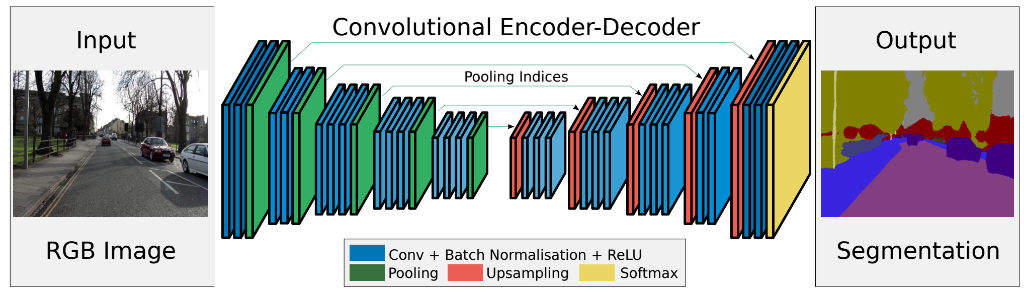
\includegraphics[scale=0.45]{images/ch3/cnn-cnn.png}
    \caption{Convolutional encoder-decoder for image segmentation in the SeqNet architecture \citep{Badrinarayanan2017}}
    \label{fig:cnn-cnn}
\end{figure}

Encoder-decoder networks based on RNN are very common in problems requiring \textit{sequence-to-sequence (seq2seq)} modeling, such as translation, summarising and question-answering. For example, \cref{fig:rnn-rnn} shows an example of a model used to generate automatic responses to incoming emails. The left half of the network encodes the email into a feature vector, and the right half of the network decodes the feature vector to produce word predictions. 

\begin{figure}[hpt]
    \centering
    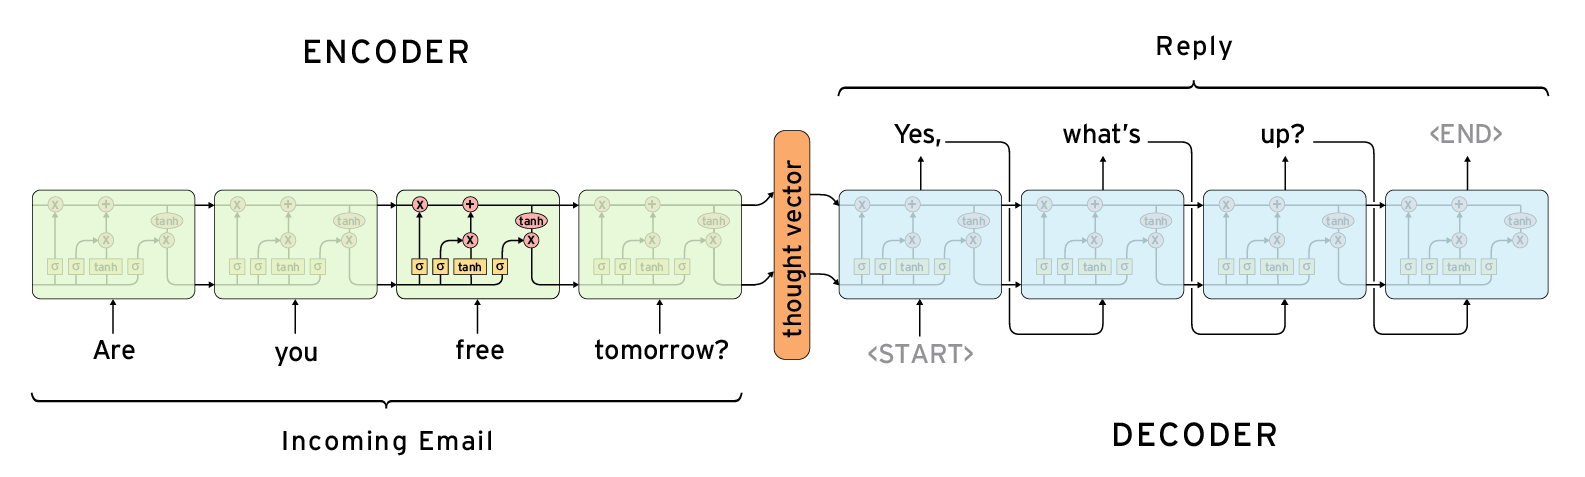
\includegraphics[scale=0.3]{images/ch3/rnn-rnn.png}
    \caption{Recurrent encoder-decoder for automated email answering. The model is given input a sentence and produces a response in the same language. Source: \href{https://ai.googleblog.com/2015/11/computer-respond-to-this-email.html}{Google AI Blog}}
    \label{fig:rnn-rnn}
\end{figure}

However, in general, an encoder-decoder network may hybridize different types of network. A common pattern is the CNN-RNN architecture, which uses a CNN as the encoder and an RNN as the decoder. This is a class of models that is both spatially and temporally deep and has the flexibility to be applied to a variety of multimodal tasks involving visual inputs and sequential outputs. Some examples of tasks where this architecture is used include:

\begin{itemize}
    \item Visual time series forecasting: Predicting the evolution of series, such as stock prices or energy load.
    \item Activity recognition: Generating a textual description of an activity demonstrated in a sequence of images.
    \item Image captioning: Generating a textual description of a single image.
    \item Video description: Generating a textual description of a sequence of images.
\end{itemize}

This architecture was originally referred to as a Long-term Recurrent Convolutional Network (LRCN) \citep{Donahue2015}, since typically it uses LSTM for the recurrent part. For example, \cref{fig:cnn-rnn} depicts the Neural Image Captioner developed by Google \citep{Vinyals2015}, which uses a Batch Normalization version of their Inception CNN for the encoder and an LSTM network for the decoder. The model works as follows: first, the CNN process an image and extracts visual features, which are then passed as input to the LSTM. The LSTM takes a word, the context from previous time steps, and defines a probability distribution over the next word in the sentence. The LSTM is conditioned on the image information at the first time step. The generative process is started with a special "<start>" token and ends when a special "<end>" token is generated.

\begin{figure}[hpt]
    \centering
    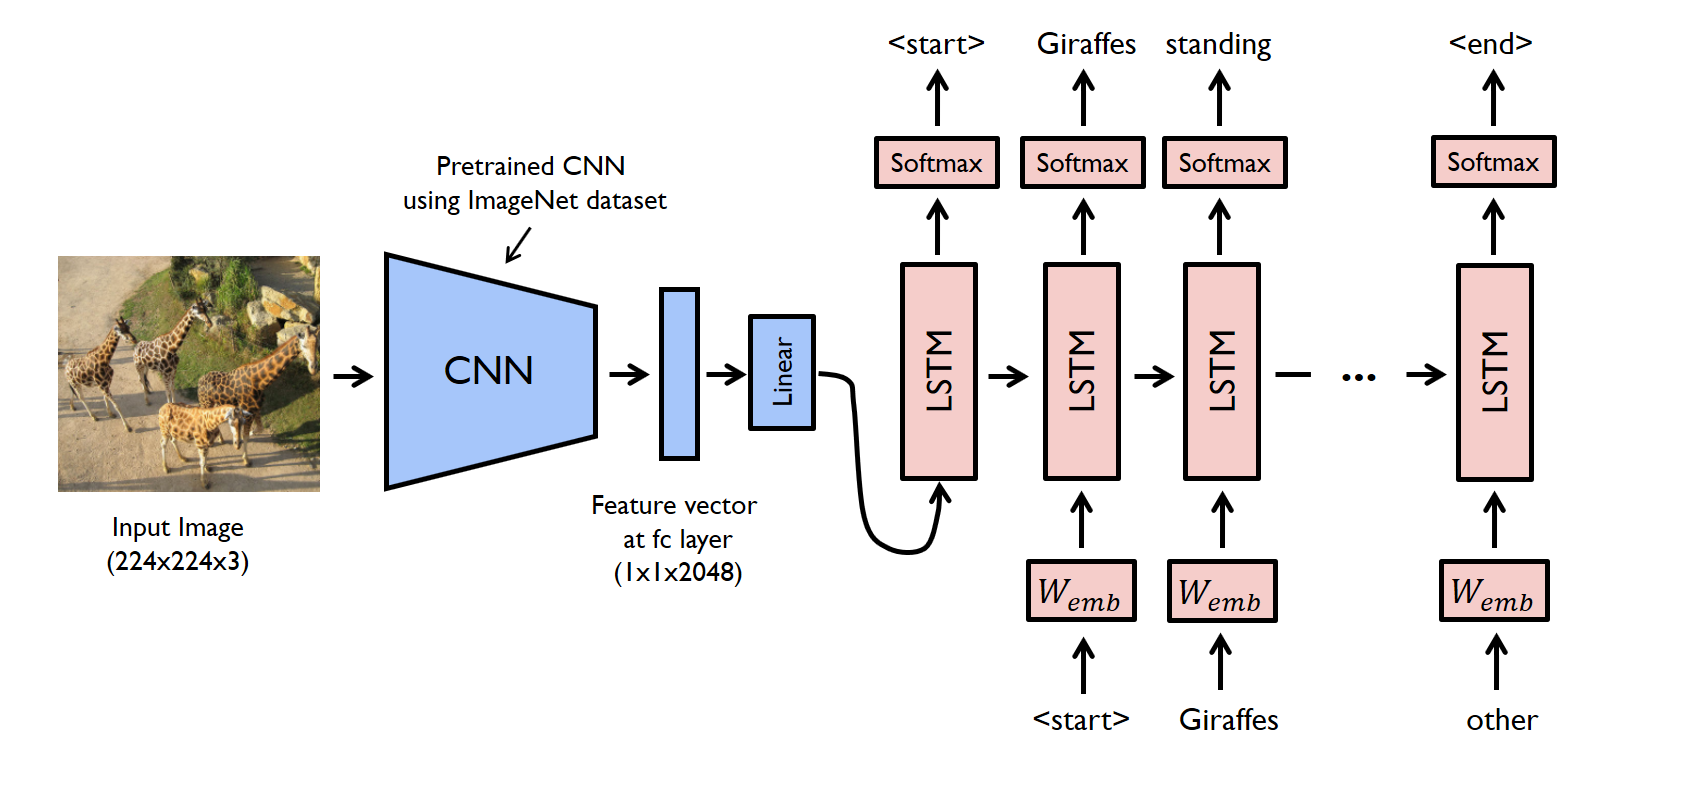
\includegraphics[scale=0.3]{images/ch3/cnn-rnn.png}
    \caption{Encoder-decoder combining CNN and LSTM for image captioning. Source:  \href{https://github.com/yunjey/pytorch-tutorial/tree/master/tutorials/03-advanced/image_captioning}{Yunjey Choi's implementation} of the \textit{Show and Tell} model \citep{Vinyals2015}.}
    \label{fig:cnn-rnn}
\end{figure}

A key of this architecture is the use of a CNN that is pre-trained on a challenging image classification task, which is re-purposed as a feature extractor for the caption generating problem (this is called \textit{transfer learning}). Typically, a CNN trained on the ImageNet dataset is used for this purpose.

For the decoder, most systems proposed so far use LSTM units, since they are more powerful than other types of recurrent units, although lately, GRU units have also emerged as a viable alternative with similar capabilities bu reduced cost.

\subsection{Sequence to Sequence  modelling}\label{subsec:seq2seq}

Next, we delve into the case where both the encoder and decoder are recurrent networks and is commonly known as sequence-to-sequence modeling.

\paragraph{Seq2seq architecture}
Sequence to sequence modeling, \textit{seq2seq} for short, is based on the encoder-decoder architecture to generate a sequence output for a sequence input. This model was born in the field of language modeling \citep{Sutskever2014}. Broadly speaking, it aims to transform an input sequence (source) to a new one (target) and both sequences can be of arbitrary lengths. Examples of transformation tasks include machine translation between multiple languages in either text or audio, question-answer dialog generation, or even parsing sentences into grammar trees.

The seq2seq model normally has an encoder-decoder architecture, composed of:
\begin{itemize}
    \item An encoder processes the input sequence and compresses the information into a context vector (also known as sentence embedding or “thought” vector) of a fixed length. This representation is expected to be a good summary of the meaning of the whole source sequence.
    \item A decoder is initialized with the context vector to emit the transformed output. The early work only used the last state of the encoder network as the decoder initial state.
\end{itemize}    

Both the encoder and decoder are recurrent neural networks, i.e. using LSTM or GRU units


\cref{fig:rnn-rnn} shows an example of a query answering application that uses the seq2seq model. \cref{fig:seq2seq} shows another example of seq2seq modeling applied to translation.

\begin{figure}[hpt]
    \centering
    \includesvg{images/ch3/seq2seq.svg}
    \caption{The sequence to sequence model architecture.}
    \label{fig:seq2seq}
\end{figure}

The layers in the encoder and the decoder are illustrated in \cref{fig:seq2seq_details}.

\begin{figure}[hpt]
    \centering
    \includesvg{images/ch3/seq2seq-details.svg}
    \caption{Layers in seq2seq model.}
    \label{fig:seq2seq_details}
\end{figure}

\paragraph{Seq2seq encoder}
In the encoder, we use the word embedding layer to obtain a feature index from the word index of the input language and then input it into a multi-level recurrent layer, typically made of gated recurrent units such as LSTM or GRU. The input for the encoder is a batch of sequences, which is 2-D tensor with shape (batch size, sequence length). The output consists of both the outputs of the recurrent units and the hidden states (and memory cells of the last time step if using LSTM).

The output shape returned by the encoder after performing forward calculation on the input is (number of time steps, batch size, number of hidden units). The shape of the multi-layer hidden state of the gated recurrent unit in the final time step is (number of hidden layers, batch size, number of hidden units). If GRU is used the \textit{state}  contains only one element, which is the hidden state. If LSTM is used, the \textit{state} list will also contain another element, which is the memory cell.

\paragraph{Seq2seq decoder}
We directly use the hidden state of the encoder in the final time step as the initial hidden state of the decoder. This requires that the encoder and decoder RNNs have the same numbers of layers and hidden units.

The forward calculation of the decoder is similar to the encoder's calculation. The only difference is the addition of a dense layer with the hidden size to be the vocabulary size to output the predicted confidence score for each word.

\paragraph{Seq2seq training}

For each time step, the decoder outputs a vocabulary size confident score vector to predict words. Similar to language modeling, we can apply \textit{softmax} to obtain the probabilities and then use cross-entropy loss to calculate the loss. 

But note that we padded the target sentences to make them have the same length. We would not like to compute the loss on the padding symbols. To solve that, a masked version of the loss function is used.

During training, if the target sequence has length $n$, we feed the first $n-1$ tokens into the decoder as inputs, and the last $n-1$ tokens are used as ground truth label. This is called \textit{Teacher Forcing}, and is depicted in \cref{fig:seq2seq}.

\paragraph{Seq2sea prediction}

To predict a new sequence, the generation process is started by feeding the same "<bos>" token to the decoder at time step 0,  exactly as is done in the training stage. But the input token for a later time step is the predicted token from the previous time step, instead of the ground truth token used during training with the Teacher forcing algorithm. This process is shown in \cref{fig:seq2seq_predict}.

\begin{figure}[hpt]
    \centering
    \includesvg{images/ch3/seq2seq_predict.svg}
    \caption{Sequence to sequence model predicting with greedy search.}
    \label{fig:seq2seq_predict}
\end{figure}

Various approaches exist to predict the next token. For example, in Greedy search, the token with the highest score at each time step is chosen and used to predict the next token. More details on this will be provided in the next chapter when describing our own model details.

\subsection{Attention mechanisms}

A recent trend in Deep Learning is the use of attention mechanisms, typically added to the decoder in an encoder-decoder architecture. 

Attention is, to some extent, motivated by how we pay visual attention to different regions of an image or correlate words in one sentence. Human visual attention is well-studied and while there exist different models, all of them essentially come down to being able to focus on a certain region of an image with "high resolution" while perceiving the surrounding image in "low resolution", and then adjusting the focal point over time. Given a small patch of an image, pixels in the rest provide clues about what should be displayed there. For example, if we see an eye besides a nose, we expect to see another eye at the opposite side of the nose. Similarly, we can explain the relationship between words in one sentence or a close context. When we see "eating", we expect to encounter a food word very soon. 

Attention in Neural Networks has a long history, particularly in image recognition, but only recently have attention mechanisms made their way into recurrent neural networks architectures that are typically used in NLP, and increasingly also in computer vision tasks.

\subsubsection{Attention in Neural Machine Translation}

In the original seq2seq model (\cref{subsec:seq2seq}), the source sequence is encoded into a fixed length context vector that is then passed to the decoder to generate a target sequence. A critical and apparent disadvantage of the fixed-length context vector design of the initial seq2seq model lies in its incapability of remembering long sentences. Often it has forgotten the first part once it completes processing the whole input. The attention mechanism was proposed by \citet{Bahdanau2015} to resolve this weakness. 

Besides, often, a token in the target sequence may closely relate to some tokens in the source sequence instead of the whole source sequence. For example, when translating "Hello world." to "Bonjour le monde.", "Bonjour" maps to "Hello" and "monde" maps to "world".  In the seq2seq model, the decoder may implicitly select the corresponding information from the state passed by the decoder. The attention mechanism, however, makes this selection explicit.

Below we describe the attention mechanism as originally proposed by \citeauthor{Bahdanau2015}, and then we will present a more general model of attention which can be applied to multimodal information tasks such as image captioning, which combines both visual and textual information.

The attention mechanism was born to help memorize long source sentences in neural machine translation (NMT). Rather than building a single context vector out of the encoder’s last hidden state, the secret sauce invented by attention is to create shortcuts between the context vector and the entire source input. The weights of these shortcut connections are customizable for each output element.

While the context vector has access to the entire input sequence, we don’t need to worry about forgetting. The alignment between the source and target is learned and controlled by the context vector. Essentially the context vector consumes three pieces of information: encoder hidden states, decoder hidden states, and alignment between source and target.

\begin{figure}[hpt]
    \centering
    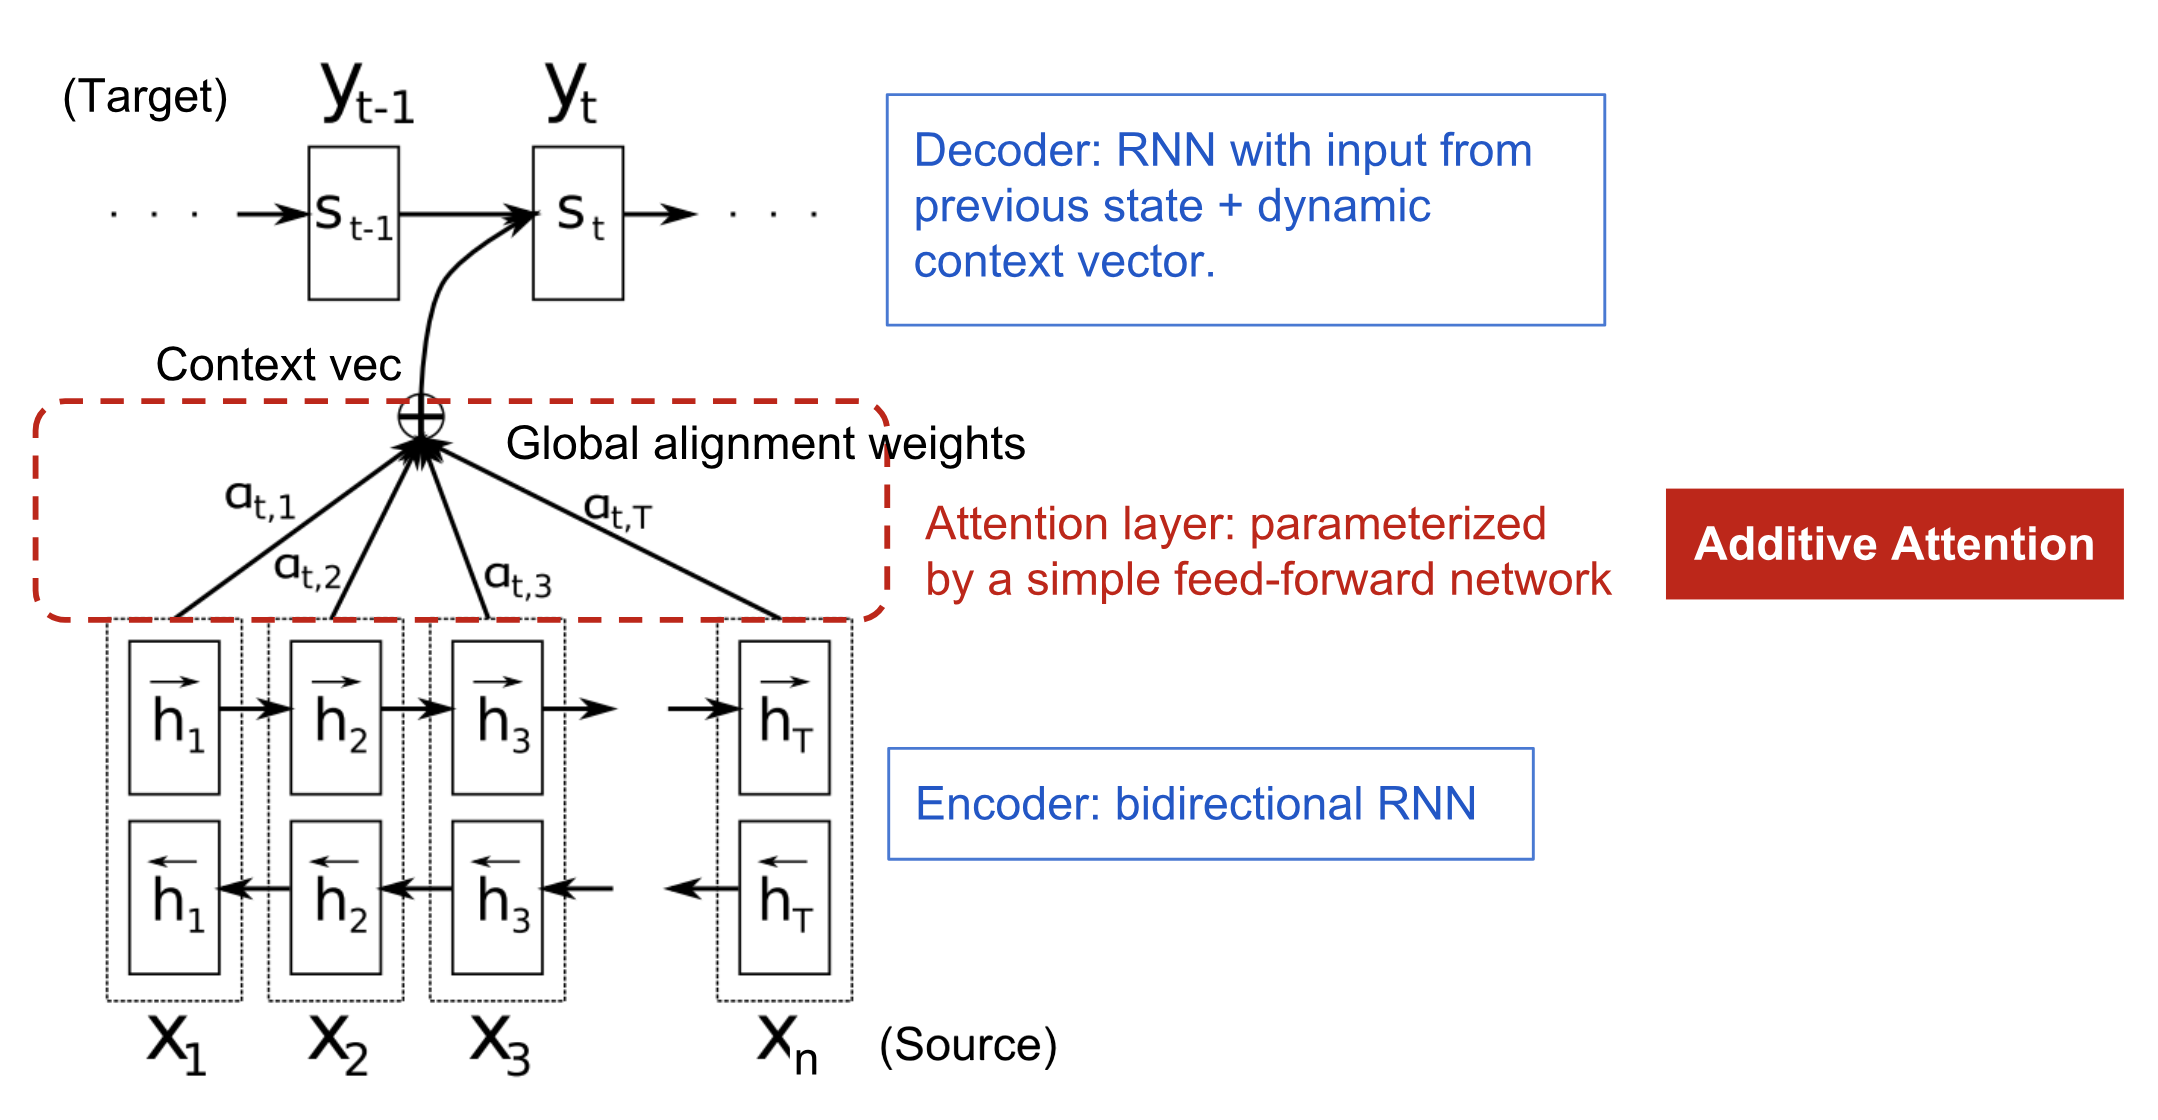
\includegraphics[scale=0.35]{images/ch3/bahdanau-attention.png}
    \caption{The encoder-decoder model with additive attention mechanism in \citep{Bahdanau2015}}
    \label{fig:bahdanau-attention}
\end{figure}

More formally: say, we have a source sequence $\mathbf{x}$ of length $n$ and try to output a target sequence $\mathbf{y}$ of length $m$:
$$
\begin{aligned}
\mathbf{x} &= [x_1, x_2, \dots, x_n] \\
\mathbf{y} &= [y_1, y_2, \dots, y_m]
\end{aligned}
$$
(Variables in bold indicate that they are vectors; same for everything else in this post.)

The encoder is a bidirectional RNN (or any other recurrent network setting of your choice) with a forward hidden state $\overrightarrow{\boldsymbol{h}}_i$ and a backward one $\overleftarrow{\boldsymbol{h}}_i$. A simple concatenation of two represents the encoder state. The motivation is to include both the preceding and following words in the annotation of one word.

$$
\boldsymbol{h}_i = [\overrightarrow{\boldsymbol{h}}_i^\top; \overleftarrow{\boldsymbol{h}}_i^\top]^\top, i=1,\dots,n
$$

The decoder network has hidden state $\boldsymbol{s}_t=f(\boldsymbol{s}_{t-1}, y_{t-1}, \mathbf{c}_t)$ for the output word at position $t, t=1,\dots,m$, where the context vector $\mathbf{c}_t$ is a sum of hidden states of the input sequence, weighted by alignment scores:
$$
\begin{aligned}
\mathbf{c}_t &= \sum_{i=1}^n \alpha_{t,i} \boldsymbol{h}_i & \small{\text{; Context vector for output }y_t}\\
\alpha_{t,i} &= \text{align}(y_t, x_i) & \small{\text{; How well two words }y_t\text{ and }x_i\text{ are aligned.}}\\
&= \frac{\exp(\text{score}(\boldsymbol{s}_{t-1}, \boldsymbol{h}_i))}{\sum_{i'=1}^n \exp(\text{score}(\boldsymbol{s}_{t-1}, \boldsymbol{h}_{i'}))} & \small{\text{; Softmax of some predefined alignment score.}}.
\end{aligned}
$$

The alignment model assigns a score $\alpha_{t,i}$ to the pair of input at position i and output at position $t, (y_t, x_i)$, based on how well they match. The set of $\{\alpha_{t, i}\}$ are weights defining how much of each source hidden state should be considered for each output. In \citep{Bahdanau2015}, the alignment score $\alpha$ is parameterized by a feed-forward network with a single hidden layer and this network is jointly trained with other parts of the model. The score function is therefore in the following form, given that \textit{tanh} is used as the non-linear activation function:

$$\text{score}(\boldsymbol{s}_t, \boldsymbol{h}_i) = \mathbf{v}_a^\top \tanh(\mathbf{W}_a[\boldsymbol{s}_t; \boldsymbol{h}_i])$$

where both $\mathbf{v}_a$ and $\mathbf{W}_a$ are weight matrices to be learned in the alignment model.

The matrix of alignment scores is a nice byproduct to explicitly show the correlation between source and target words.

\begin{figure}[hpt]
    \centering
    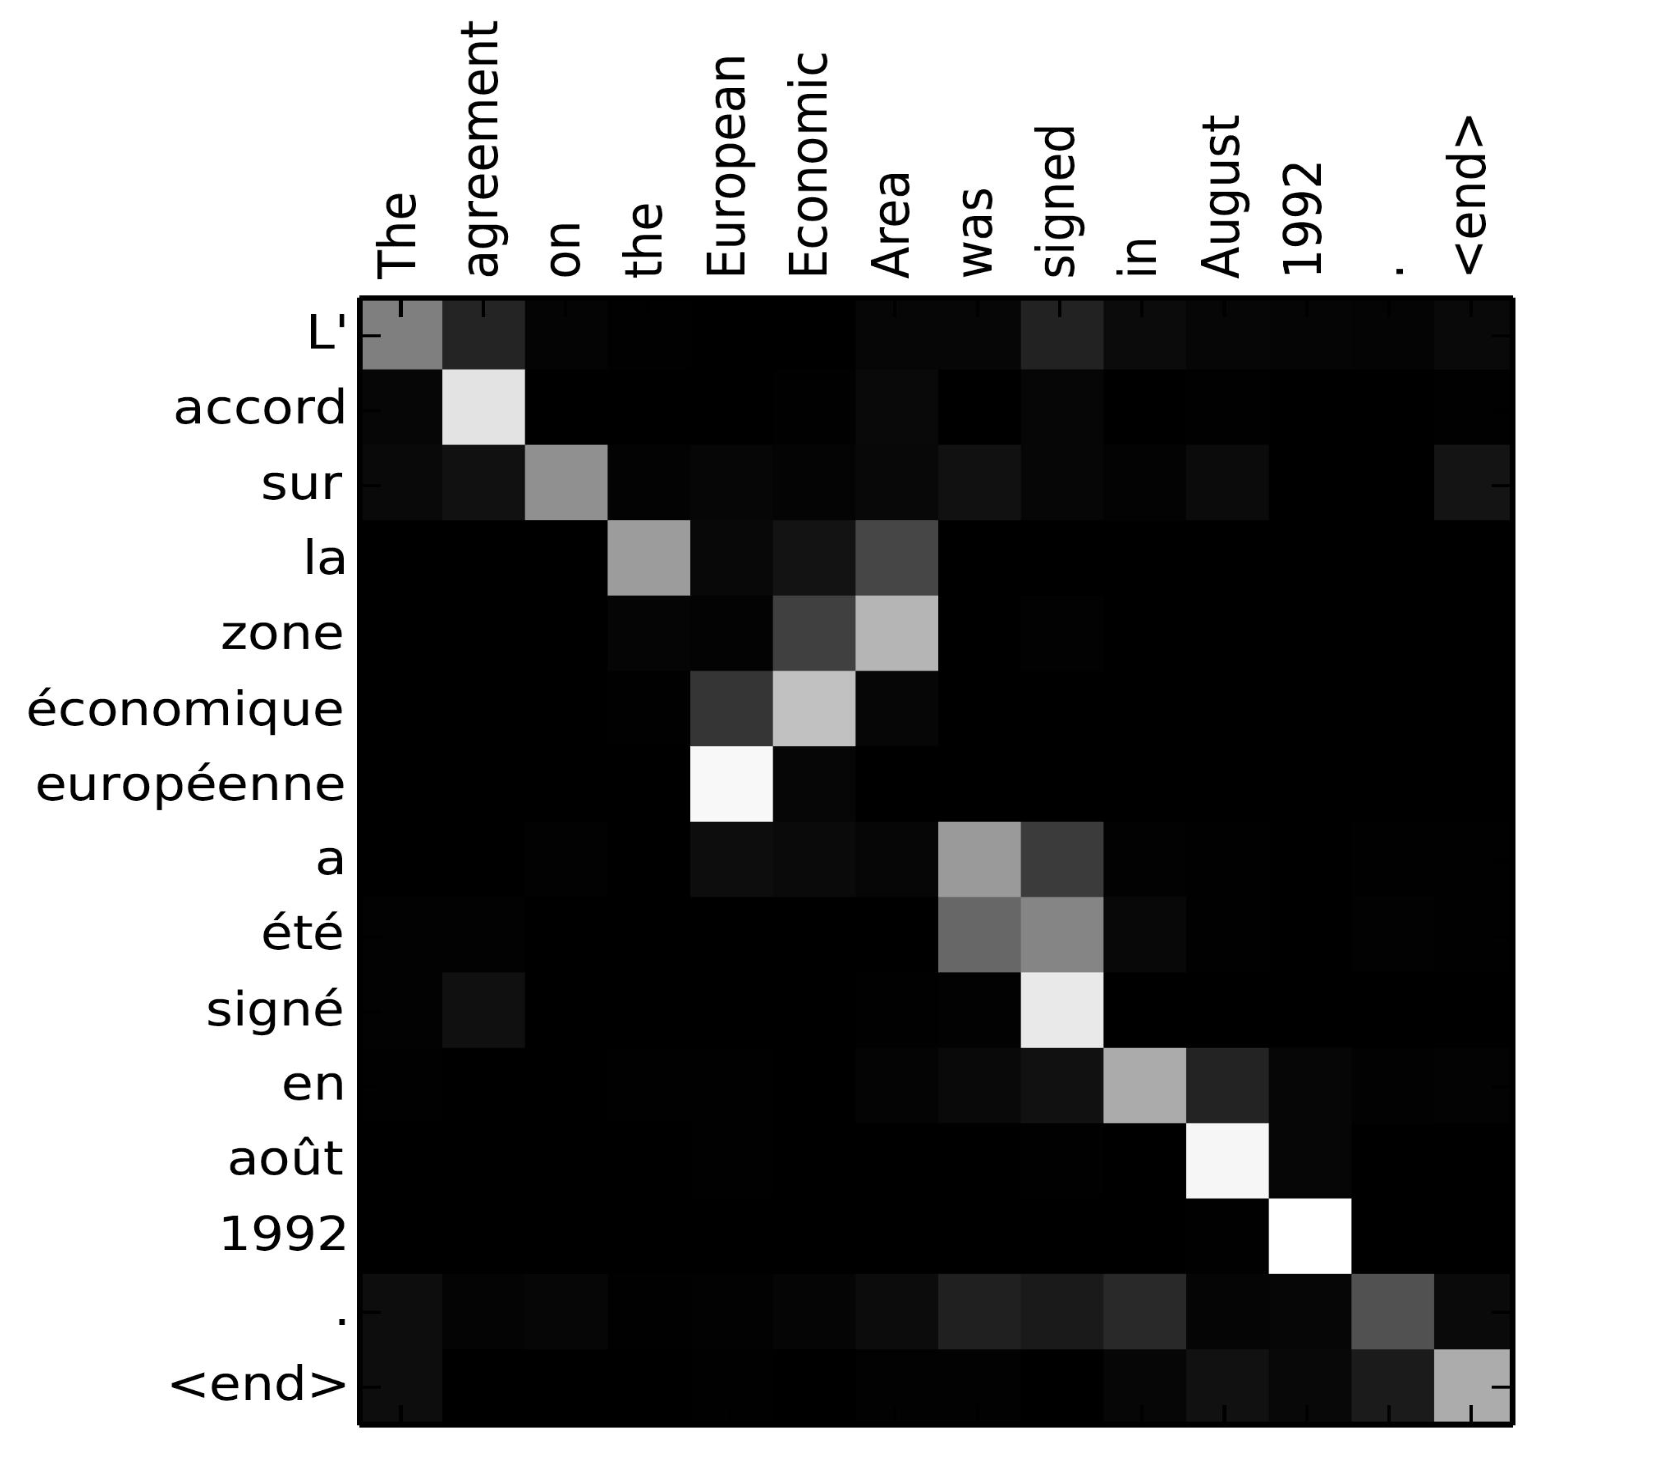
\includegraphics[scale=0.3]{images/ch3/alignment-matrix.png}
    \caption{Alignment matrix of an French sentence and its English translation. Source: Fig 3 in \citep{Bahdanau2015})}
    \label{fig:alignment-matrix}
\end{figure}

\subsubsection{Different attention mechanisms}

With the help of the attention, the dependencies between source and target sequences are not restricted by the in-between distance anymore. Given the big improvement by attention in machine translation, it soon got extended into the computer vision field \citep{Xu2015} and people started exploring various other forms of attention mechanisms \citep{Luong2015, Britz2017, Vaswani2017}.

\cref{tab:attention-mechanisms} enumerates popular attention mechanisms and their corresponding alignment score functions, where $\mathbf{W}_a$ is a trainable weight matrix in the attention layer. 

\begin{table}[hpt]
\caption{summary table of several popular attention mechanisms and corresponding alignment score functions}
\label{tab:attention-mechanisms}
\begin{tabular}{cll}
Name & Alignment score function & Citation \\
\hline
Content-based att. & $\text{score}(\boldsymbol{s}_t, \boldsymbol{h}_i) = \text{cosine}[\boldsymbol{s}_t, \boldsymbol{h}_i]$ & \citep{Graves2014} \\
Additive & $\text{score}(\boldsymbol{s}_t, \boldsymbol{h}_i) = \mathbf{v}_a^\top \tanh(\mathbf{W}_a[\boldsymbol{s}_t; \boldsymbol{h}_i])$ & \citep{Bahdanau2015} \\
Location-Base & $\alpha_{t,i} = \text{softmax}(\mathbf{W}_a \boldsymbol{s}_t)$ & \citep{Luong2015} \\
General & $\text{score}(\boldsymbol{s}_t, \boldsymbol{h}_i) = \boldsymbol{s}_t^\top\mathbf{W}_a\boldsymbol{h}_i$ & \citep{Luong2015} \\
Dot-Product & $\text{score}(\boldsymbol{s}_t, \boldsymbol{h}_i) = \boldsymbol{s}_t^\top\boldsymbol{h}_i$ & \citep{Luong2015} \\
Scaled Dot-Product & $\text{score}(\boldsymbol{s}_t, \boldsymbol{h}_i) = \frac{\boldsymbol{s}_t^\top\boldsymbol{h}_i}{\sqrt{n}}$  & \citep{Vaswani2017}
\end{tabular}
\end{table}

\paragraph{Notes} \textit{Additive} attention is also referred to as \textit{additive} or \textit{concat} by other authors. \textit{Location-based} attention simplifies the softmax alignment to only depend on the target position. The \textit{scaled dot attention} is very similar to the dot-product attention except for the scaling factor $1/\sqrt{n}$; where $n$ is the dimension of the source hidden state.

Besides the scoring functions, there are different ways to classify attention mechanisms, for example:

\begin{itemize}
    \item Self-Attention \citep{Cheng2016}: Relating different positions of the same input sequence. Theoretically, the self-attention mechanism can adopt any score functions above, but just replace the target sequence with the same input sequence. 
    \item Global/Soft \cite{Xu2015}: Attending to the entire input state space. 
    \item Local/Hard \citep{Xu2015, Luong2015}: Attending to the part of input state space; i.e. a patch of the input image.
\end{itemize}

\subsubsection{Self-Attention}

Self-attention, also known as intra-attention, is an attention mechanism relating different positions of a single sequence in order to compute a representation of the same sequence. It has been shown to be very useful in machine reading, abstractive summarization, or image description generation.

The LSTM network by \citet{Cheng2016} uses self-attention to do machine reading. \cref{fig:self-attention} illustrates this mechanism with an example. See how self-attention mechanism enables the model to learn the correlation between the current words and the previous part of the sentence.

\begin{figure}[hpt]
    \centering
    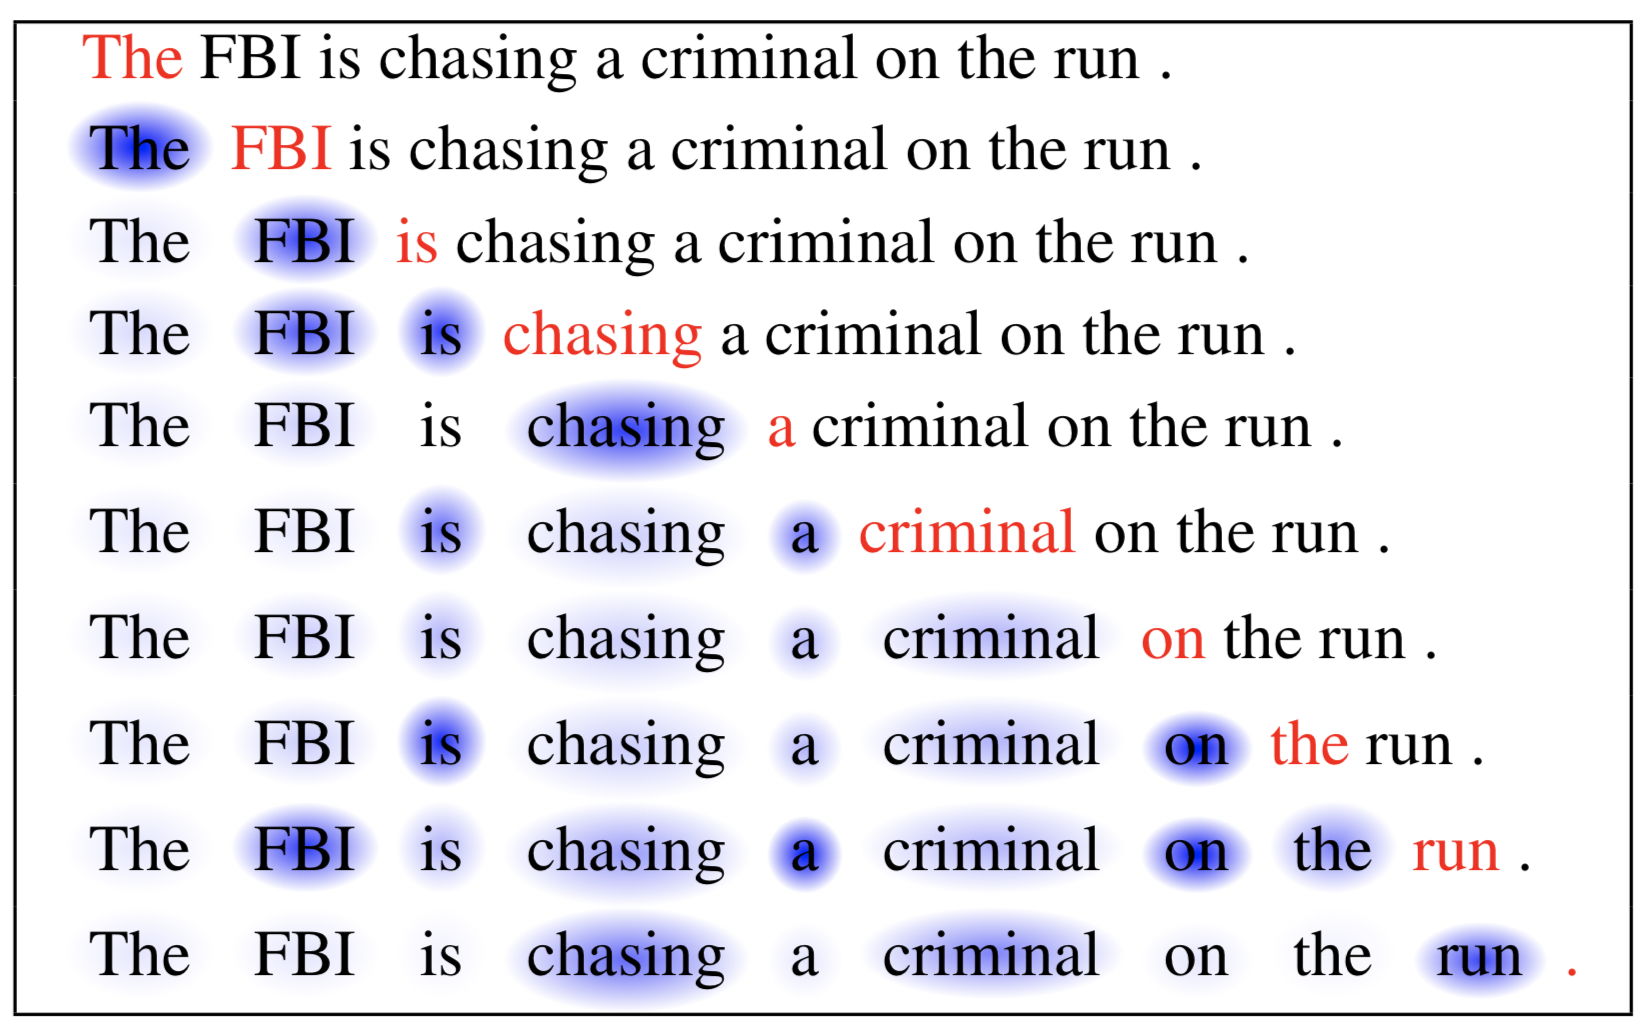
\includegraphics[scale=0.2]{images/ch3/self-attention.png}
    \caption{The current word is in red and the size of the blue shade indicates the activation level. Source: \citep{Cheng2016}.}
    \label{fig:self-attention}
\end{figure}

Self-attention can also be applied to image captioning. For example, in the "Show, attend and tell" paper by \citet{Xu2015}, an input image is first encoded by a convolutional neural network to generate a feature map, and then a recurrent network with self-attention over the image consumes the attention-weighted feature maps to generate the descriptive words one by one. The visualization of the attention weights clearly demonstrates which regions of the image the model pays attention to so as to output a certain word.

\begin{figure}[hpt]
    \centering
    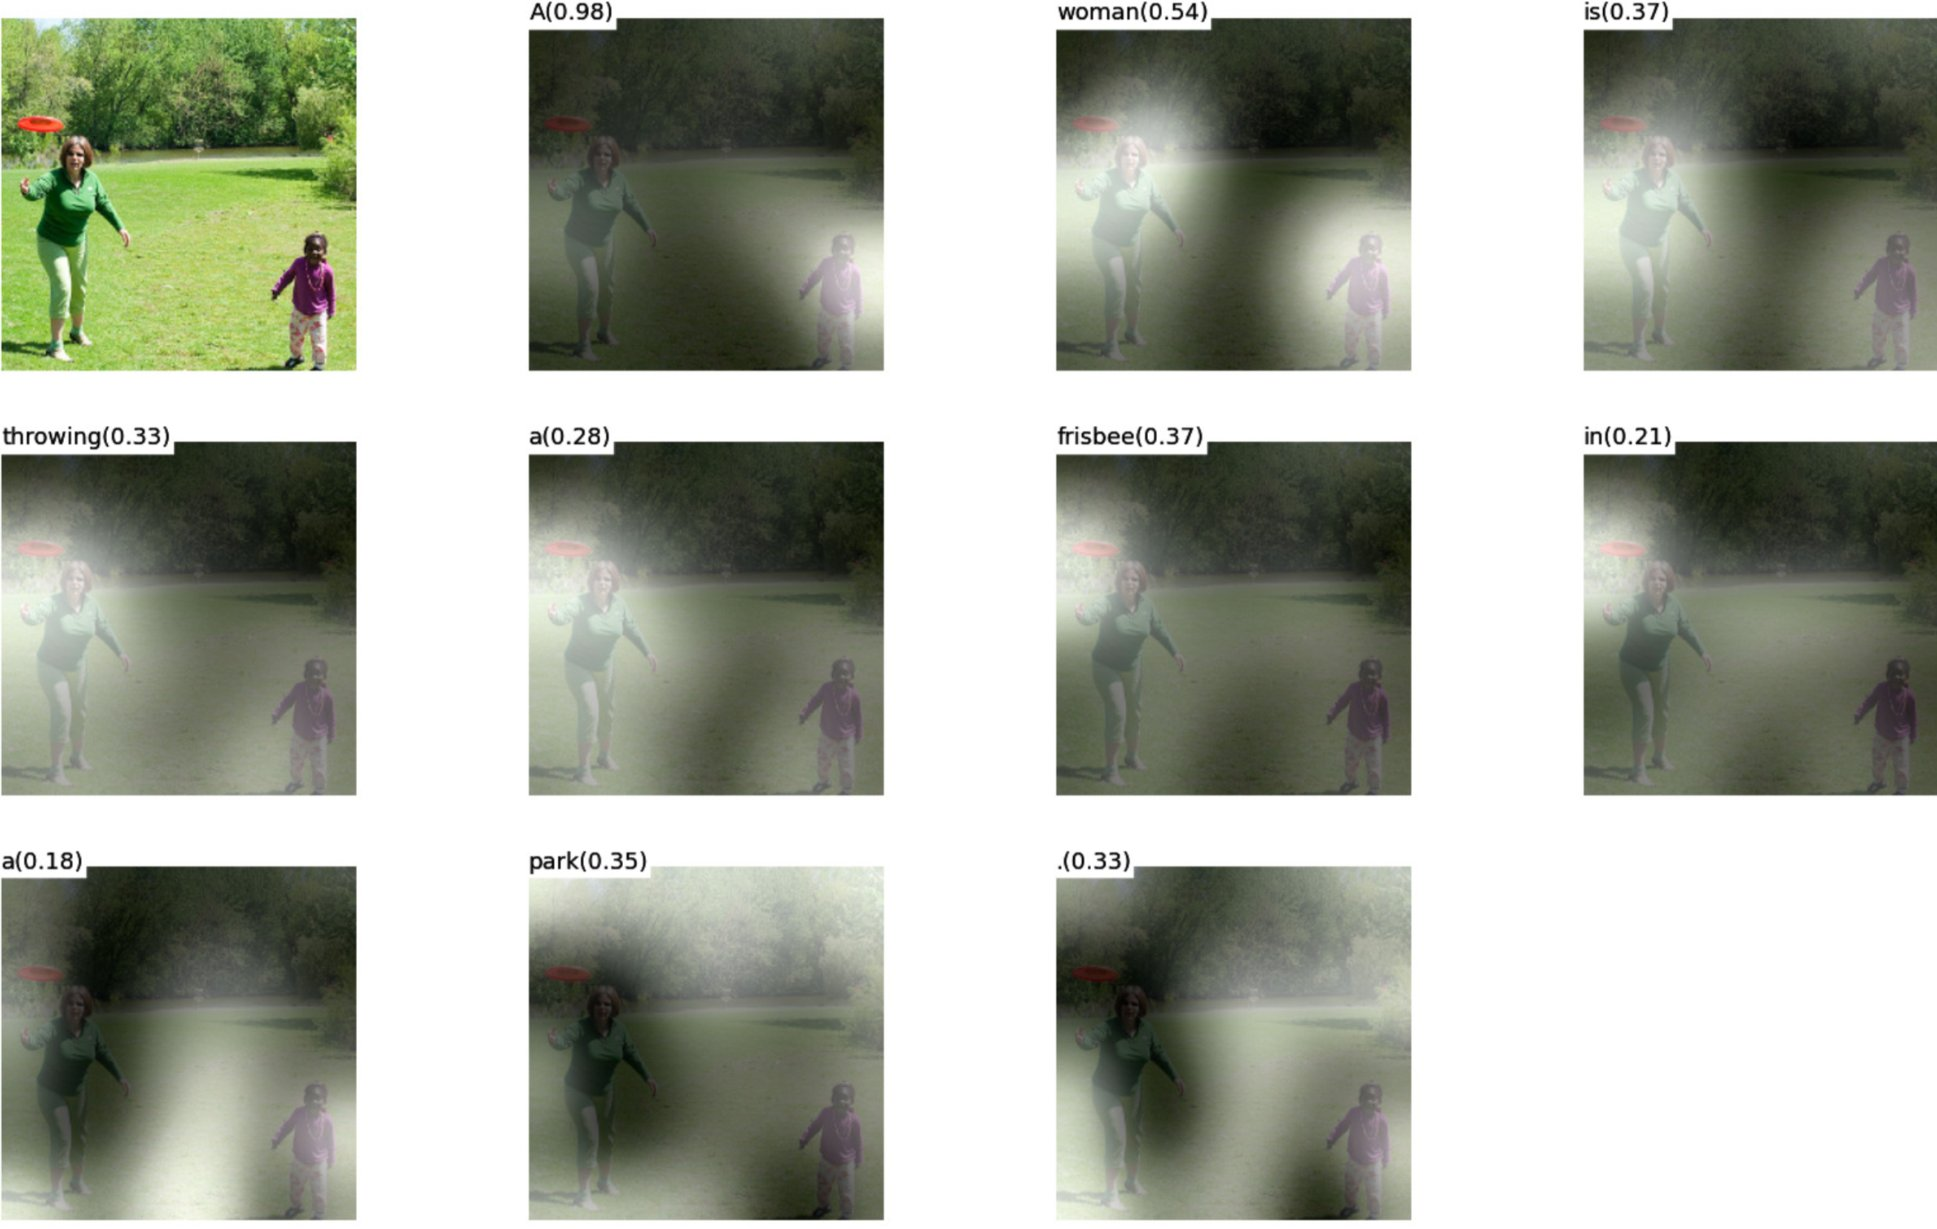
\includegraphics[scale=0.2]{images/ch3/visual-attention.jpg}
    \caption{Caption generation example:A woman is throwing a frisbee in a park. Source: \citep{Xu2015}.}
    \label{fig:visual-attention}
\end{figure}

\subsubsection{Soft vs Hard Attention}

The \textit{soft} vs \textit{hard} attention is another way to categorize how attention is defined. The original idea was proposed in the "Show, attend and tell" paper \citep{Xu2015}, based on whether the attention has access to the entire image or only a patch:

\begin{itemize}
    \item Soft Attention: the alignment weights are learned and placed "softly" over all patches in the source image; which corresponds to the additive attention model by \citet{Bahdanau2015}.
    \begin{itemize}
        \item Pro: the model is smooth and differentiable.
        \item Con: expensive when the source input is large.
    \end{itemize}
    \item Hard Attention: only selects one patch of the image to attend to at a time.
    \begin{itemize}
        \item Pro: less calculation at the inference time.
        \item Con: the model is non-differentiable and requires more complicated techniques such as variance reduction or reinforcement learning to train \citep{Luong2015}. 
    \end{itemize}
\end{itemize}

\cref{fig:soft-vs-hard-attention} illustrates the soft vs hard effect attention with a visual example from the original paper.

\begin{figure}[hpt]
    \centering
    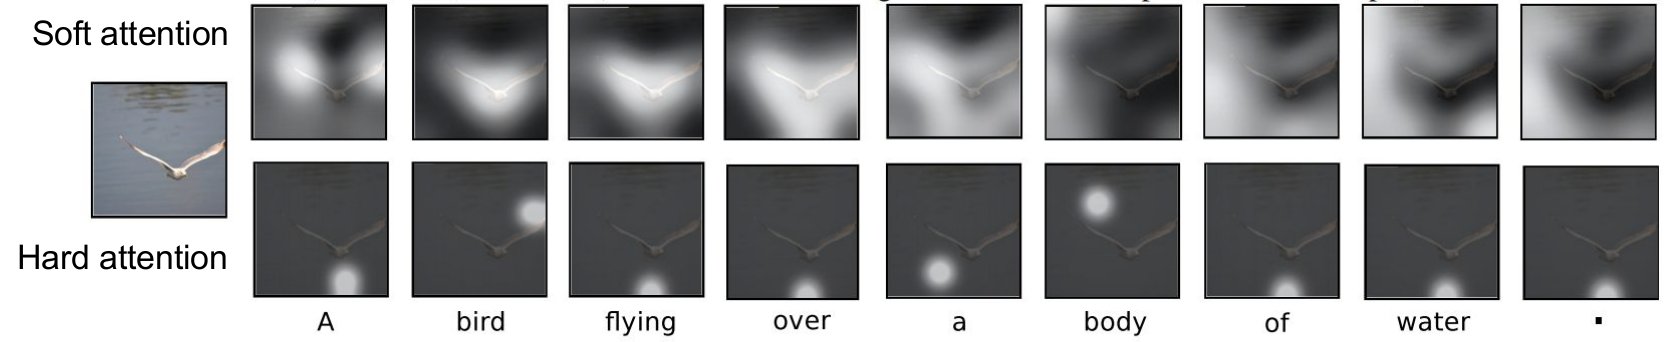
\includegraphics[scale=0.3]{images/ch3/soft-vs-hard-attention.png}
    \caption{Comparative of soft (top) vs hard (bottom) attention during caption generation. Source: \citep{Xu2015}.}
    \label{fig:soft-vs-hard-attention}
\end{figure}

\subsubsection{Global vs Local Attention}

\citet{Luong2015} coined the \textit{global} vs \textit{local} attention distinction. The global attention is similar to the soft attention, while the local one is an interesting blend between hard and soft, an improvement over the hard attention to make it differentiable: the model first predicts a single aligned position for the current target word and a window centered around the source position is then used to compute a context vector.

\cref{fig:global-vs-local-attention} compares global and local models of attention in a seq2seq setup.

\begin{figure}[hpt]
    \centering
    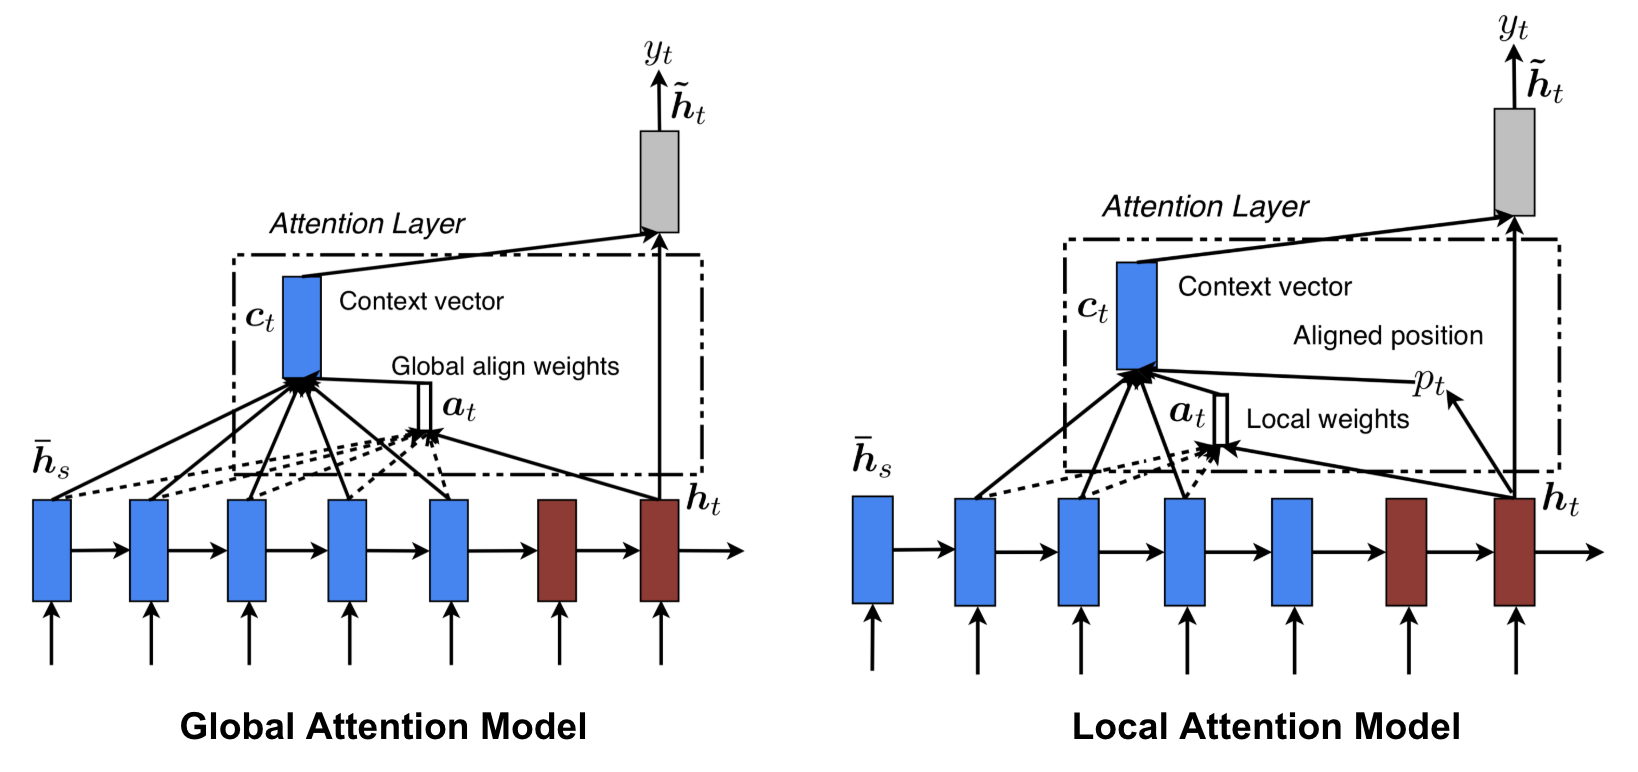
\includegraphics[scale=0.3]{images/ch3/global-vs-local-attention.png}
    \caption{Comparative of global (left) vs local (right) attention in the seq2seq model. Source: \citep{Luong2015}.}
    \label{fig:global-vs-local-attention}
\end{figure}

The are other models that apply similar ideas and can thus be seen as variations of the same idea. We will not describe them here, but we enumerate them together:

\begin{itemize}
    \item The \textit{Neural Turing Machine}(NTM), by \citet{Graves2014}, is a model architecture for coupling a neural network with external memory storage. The memory mimics the Turing machine tape and the neural network controls the operation heads to read from or write to the tape. However, the memory in NTM is finite, and thus it probably looks more like a "Neural von Neumann Machine".
    \item In problems like sorting or traveling salesman, both input and output are sequential data. Unfortunately, they cannot be easily solved by classic seq2seq or NMT models, given that the discrete categories of output elements are not determined in advance, but depends on the variable input size. The \textit{Pointer Net} (Ptr-Net), was proposed by \citet{Vinyals2015} to address this problem when the output elements correspond to positions in an input sequence. Rather than using attention to blend hidden units of an encoder into a context vector (See Fig. 8), the Pointer Net applies attention over the input elements to pick one as the output at each decoder step.
    \item The \textit{transformer} model introduced in the "Attention is all you need" paper by \citet{Vaswani2017} is entirely built on the self-attention mechanisms without using sequence-aligned recurrent architecture. It presented a lot of improvements to the soft attention mechanism, and make it possible to do seq2seq modeling without recurrent network unit, thus reducing the computational costs.
\end{itemize}

% \subsection{A general model of attention}\label{subsec:general-attention-model}

% Formally, attention is a \textit{generalized pooling method with bias alignment over inputs}. The core component in the attention mechanism is the \textbf{attention layer}. An input of the attention layer is called a \textbf{query}. For a query, the attention layer returns the output based on its \textbf{memory}, which is a set of key-value pairs. To be more specific, assume a query $\mathbf{q}\in\mathbb R^{d_q}$, and the memory contains $n$ key-value pairs, $(\mathbf{k}_1, \mathbf{v}_1), \ldots, (\mathbf{k}_n, \mathbf{v}_n)$, with $\mathbf{k}_i\in\mathbb R^{d_k}$, $\mathbf{v}_i\in\mathbb R^{d_v}$. The attention layer then returns an output $\mathbf o\in\mathbb R^{d_v}$ with the same shape, such that each key has a value.

% \begin{figure}[hpt]
%     \centering
%     \includesvg{images/ch3/attention.svg}
%     \caption{The attention layer returns an output based on the input query and its memory.}
%     \label{fig:attention}
% \end{figure}

% To compute the output, we first assume there is a score function $\alpha$ which measures the similarity --\textit{alignment}-- between the query and a key. Then we compute all $n$ scores $a_1, \ldots, a_n$ by

% $$a_i = \alpha(\mathbf q, \mathbf k_i).$$

% Next we use \textit{softmax} to obtain the attention weights

% $$b_1, \ldots, b_n = \textrm{softmax}(a_1, \ldots, a_n).$$

% The output is then a weighted sum of the values

% $$\mathbf o = \sum_{i=1}^n b_i \mathbf v_i.$$

% Different choices of the score function lead to different attention layers, as the ones shown in \cref{tab:attention-mechanisms}. 

% Below we see how this general model fits some of the specific models introduced above, More specifically, we briefly describe two of the most popular attention models: the \textit{dot product} and the \textit{additive} models. 

% \subsubsection{Scaled Dot Product Attention}

% The dot product assumes the query has the same dimension than the keys, namely $\mathbf q, \mathbf k_i \in\mathbb R^d$ for all $i$. It computes the score by an inner product between the query and a key, and often then divided by $\sqrt{d}$ to make the scores less sensitive to the dimension $d$. In other words,

% $$\alpha(\mathbf q, \mathbf k) = \langle \mathbf q, \mathbf k \rangle /\sqrt{d}.$$

% Assume $\mathbf Q\in\mathbb R^{m\times d}$ contains $m$ queries and $\mathbf K\in\mathbb R^{n\times d}$ has all $n$ keys. We can compute all $mn$ scores by

% $$\alpha(\mathbf Q, \mathbf K) = \mathbf Q \mathbf K^T /\sqrt{d}.$$

% This attention mechanism could also include a dropout regularization mechanism (to randomly drop some attention weights).

% \subsubsection{Additive attention (Multilayer Perception)}

% Multilayer perception attention was proposed by \citet{Bahdanau2015} for seq2seq modeling. In this form of attention, we first project both query and keys into a common feature space $h$.

% To be more specific, assume learnable parameters $\mathbf W_k\in\mathbb R^{h\times d_k}$, $\mathbf W_q\in\mathbb R^{h\times d_q}$, and $\mathbf v\in\mathbb R^{p}$, then the score function is defined by

% $$\alpha(\mathbf k, \mathbf q) = \mathbf v^T \text{tanh}(\mathbf W_k \mathbf k + \mathbf W_q\mathbf q). $$

% It equals to concatenate the key and value in the feature dimension, and then feed them into a hidden-layer perception with hidden size $h$ and output size $1$. The hidden layer activation function is \textit{tanh}, and no bias is applied.

% \subsubsection{Sequence to Sequence with Additive Attention}

% In this section, we add the attention mechanism to the sequence to sequence model introduced in \cref{subsec:seq2seq} to explicitly select the state. The following figure shows the model architecture for a decoding time step. As can be seen, the memory of the attention layer consists of the encoder outputs of each time step. During decoding, the decoder output from the previous time step is used as the query, the attention output is then fed into the decoder with the input to provide attentional context information.

% \begin{figure}[hpt]
%     \centering
%     \includesvg{images/ch3/seq2seq_attention.svg}
%     \caption{The second time step in decoding for the sequence to sequence model with attention mechanism.}
%     \label{fig:seq2seq_attention}
% \end{figure}

% The layer structure in the encoder and the decoder is shown in the following figure.

% \begin{figure}[hpt]
%     \centering
%     \includesvg{images/ch3/seq2seq-attention-details.svg}
%     \caption{Layers in seq2seq model with attention.}
%     \label{fig:seq2seq-attention-details}
% \end{figure}

% For the decoder of this model, we add an MLP attention layer which has the same hidden size as the LSTM layer. The state passed from the encoder to the decoder contains three items:

% \begin{itemize}
%     \item the encoder outputs of all time steps, which are used as the attention layer's memory with identical keys and values
%     \item the hidden state of the last time step that is used to initialize the encoder's hidden state  
%     \item valid lengths of the decoder inputs so the attention layer will not consider encoder outputs for padding tokens.
% \end{itemize}

% In each time step of decoding, we use the output of the last RNN layer as the query for the attention layer. Its output is then concatenated with the input embedding vector to feed into the RNN layer. Despite the RNN layer's hidden state also contains history information from the decoder, the attention output explicitly selects the encoder outputs that are correlated to the query and suspends other non-correlated information.

% The training loss is similar to the seq2seq model because the sequences in the training dataset are relatively short. The additional attention layer doesn’t lead to a significant difference. But due to both attention layer computational overhead and we unroll the time steps in the decoder, this model is much slower than the seq2seq model without attention.


